Ho scelto di realizzare una gerarchia di entità che potesse comprendere tutti i componenti importanti ai fini della partita. L'unica caratteristica che è stata quindi scelta per l'entità più generica è solo la sua posizione (inoltre, la direzione specificata nella posizione è opzionale). Una successiva scelta di suddivisione, che è sembrata la più coerente con il dominio del gioco, ha portato a \textit{MovableEntity}, che rappresenta tutto ciò capace di compiere un movimento. A seguire sono stati specificati anche \textit{EnemyCharacter} per raggruppare i diversi tipi di nemici e \textit{LivingEntity} per quanto riguarda i personaggi con un punteggio di vita.

In seguito alla specifica di \textit{MovableEntity} ho partecipato allo sviluppo dei metodi relativi al movimento delle entità e a tutti quelli conseguentemente necessari per il controllo e la gestione dell'area di gioco.

\begin{figure}[H]
  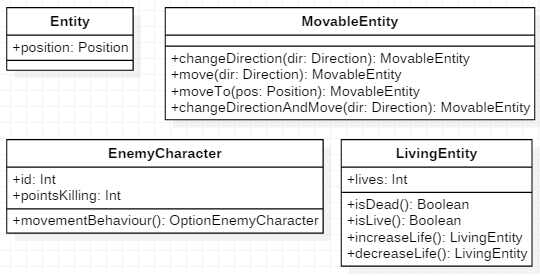
\includegraphics[width=14cm]{res/entitiesTraits.png}
  \caption{Trait delle entità del gioco}
  \label{entityTraits}
\end{figure}